\section{Application to the Global Ocean}
\label{sec:llc90}

Here we show results from a numerical implementation of the correlation model
described in \cref{sec:matern_operator}.
For this application we use the ``Lat-Lon-Cap'' (LLC) grid used by the ECCOv4
state estimate \cite[][see Sec. 2 for a complete description of the grid]{forgetECCOv4}.
The overall goal with these numerical experiments is to show that even in this
relatively complicated global grid, the
correlation model generally follows the expected Mat\'ern correlation structure
(\cref{ssec:llc90_correlations}), while maintaining
anisotropy and nonstationarity that is relevant to the physical system
(\cref{ssec:llc90_correlation_maps}).
Additionally, we show how Neumann boundary conditions to the differential
operator affect the solution in \cref{ssec:llc90_boundary_effects}.
We finish
by showing that the model can be applied efficiently with a relatively imprecise
solver tolerance (\cref{ssec:tolerance}) and that it is relatively cheap even
when the number of applications, $M$, is greater than one
(\cref{ssec:iters_and_apps}).

For all experiments, we compute statistical quantities from 1,000 samples using
the block-Successive Over Relaxation (SOR) method which is described fully in
\cref{sec:block_sor}.
Additionally, we use
$L_x(i,j) = \Delta x_g(i,j)$, $L_y(i,j) = \Delta y_g(i,j)$,
and $L_z(k) = \Delta r_f(k)$ (\cref{fig:mitgcm_grid}) where we have switched
from the spatial coordinate $\x\in\domain$ to the computational grid indices $i$, $j$, $k$.
All experiments are performed with a 3D field, which could represent an ocean
state property like temperature or salinity.

\subsection{Correspondence with theoretical correlation structure}
\label{ssec:llc90_correlations}

We first show that the sample correlation structure computed on the LLC
grid corresponds with the analytical expression for
Mat\'ern-type correlations.
For this comparison we compute the correlation field in the transformed space
$\defdomain$, where the random field can be considered isotropic and stationary.
Because we use the grid spacing to define this mapping, the correlation
distances are computed simply by counting the number of neighboring grid cells in each
direction from the point in consideration.
%We refer to this distance as $\delta\hat{x}$, $\delta\hat{y}$, and
%$\delta\hat{z}$ for the longitudinal, meridional, and vertical dimensions
%respectively.

\cref{fig:llc90_correlations} shows the comparison between the theoretically
expected correlation structure (black) and the numerically computed sample
correlation structure for
$\rangeh = \{5, 10, 15, 20\}$ (color) using $M =\{1,2,4,8\}$ (panels).
The correlation is computed in the direction of longitude, indicated by
$\delta i$.
The shading indicates the spread between the first and ninth deciles of the
sample correlation, computed at all depth levels and latitudes from
70$^\circ$S to 37$^\circ$N at 127.5$^\circ$W - a subset chosen simply to ease the
calculation.
Similar plots showing correlation in the meridional and vertical directions are
shown in the Supplemental Material.

Generally speaking, the colored curves match the analytical expression well, and
each colored curve intersects the horizontal gray line, indicating a correlation
value of 0.14, where $\rangeh = \delta i$.
We note that the largest spread in the computed correlation structure occurs
when $M=1$, especially for larger values of $\rangeh$.
Considering an analogy to Laplacian versus biharmonic damping in ocean models
\citep[e.g.][]{holland_role_1978,griffies_biharmonic_2000}, we suggest that
there is more spread when $M=1$ because the operator $\maternop^{-1}$
contains a only a Laplacian term.
Compared to the cases when $M>1$, which contain biharmonic and higher order
Laplacian terms in $\maternop^{-M}$, the Laplacian case is less
scale-selective.
That is, the operator does not cutoff higher frequency variability sharply,
allowing noise to pollute the sample statistics \citep[see][Section 2 for a quantitative
description of this cutoff in frequency space]{griffies_biharmonic_2000}.
We note, however, that the spread still allows for a reasonable interpretation
that the operator $\maternop^{-1}$ captures the behavior of the analytical Mat\'ern correlation
function.

\begin{figure}
    \centering
    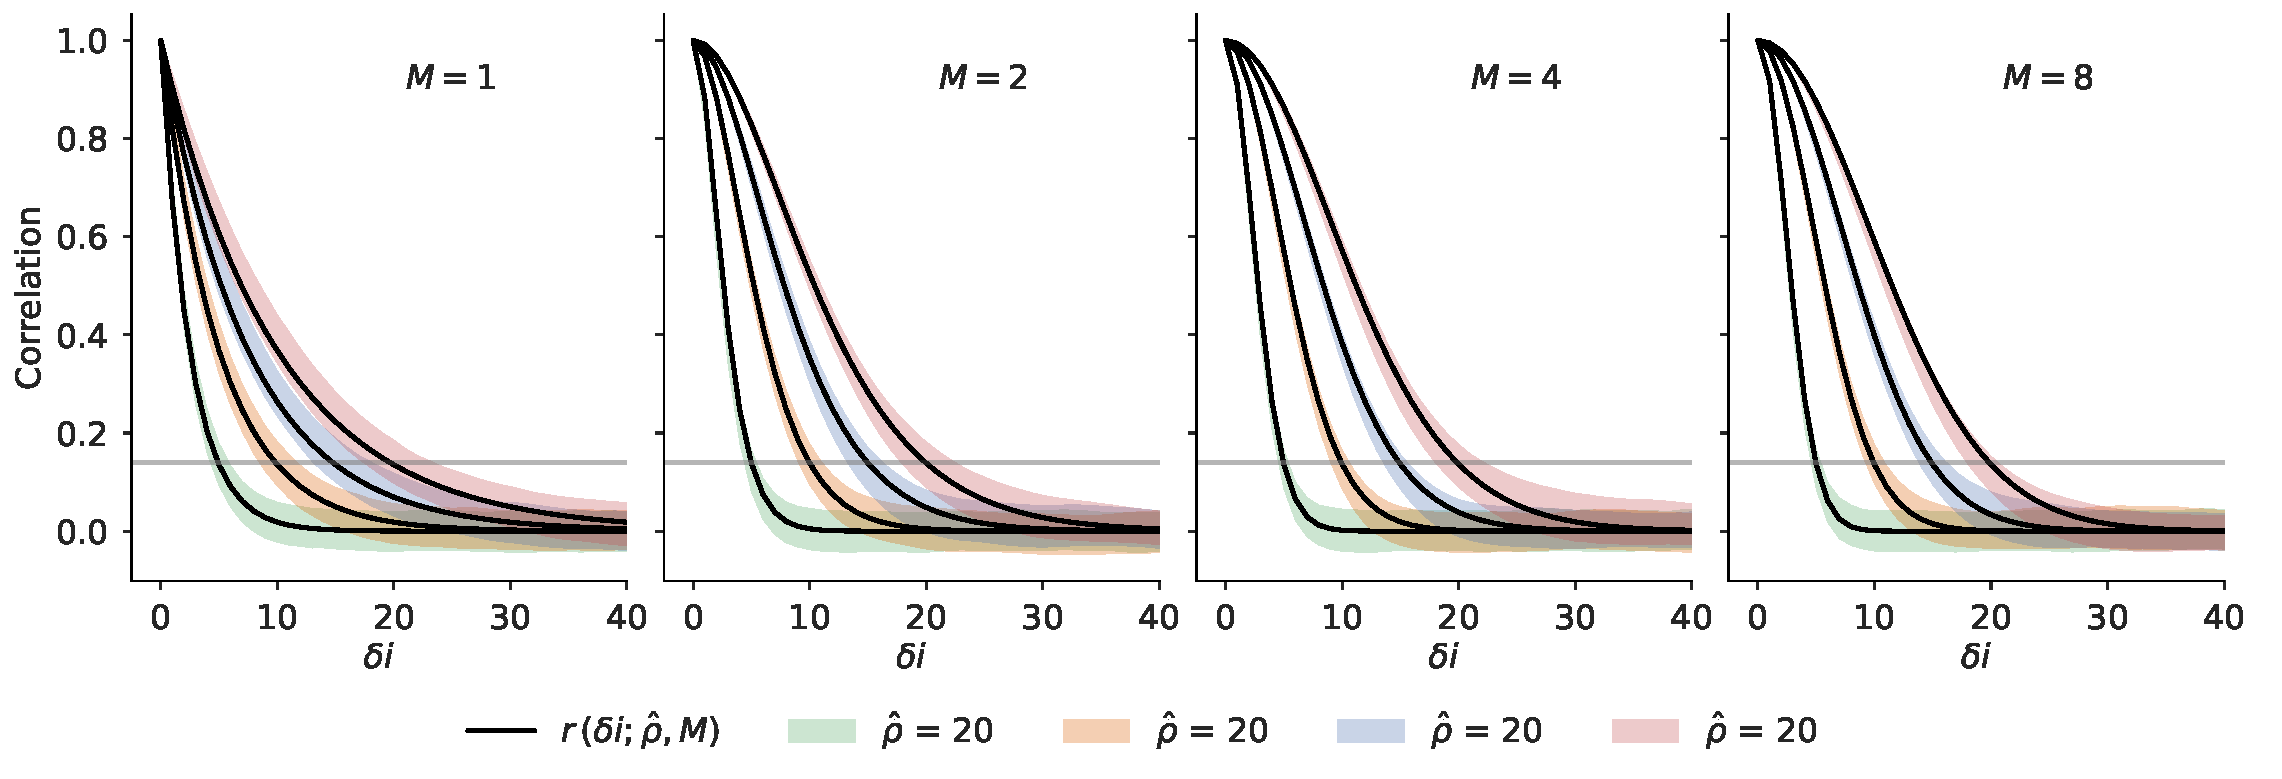
\includegraphics[width=\textwidth]{../figures/matern_llc90_correlation_theory_vs_m_ix.pdf}
    \caption{Correlation structure computed from the theoretical Mat\'ern
        correlation function (black; \cref{eq:matern_corr_isostat}) and from
        1,000 samples using a subset of the ``Lat-Lon-Cap'' grid within the
        Pacific Ocean (shaded coloring).
        The sample correlation is computed in the zonal direction, $\delta i$,
        indicating number of neighboring grid cells from
        127.5$^\circ$W.
        The shading indicates the spread between the first and ninth deciles,
        based on sample correlations at all depth levels and latitudes from
        70$^\circ$S and 37$^\circ$N.
        Similar plots showing correlation as a function of meridional and
        vertical distance are provided in the Supplemental Material.
        Sample correlation is computed from 1,000 random samples.
    }
    \label{fig:llc90_correlations}
\end{figure}

\subsection{Sample correlation maps}
\label{ssec:llc90_correlation_maps}

Maps of the sample correlation field at two locations on the LLC
grid are shown in
\cref{fig:llc90_correlation_maps}.
For these calculations we use a perhaps unrealistically large correlation length scale
defined by $\rangeh=20$ for illustrative purposes.
First, we compare panels (a) and (b) of \cref{fig:llc90_correlation_maps}, which
show the sample correlation computed at
(0.2$^\circ$N, 127.5$^\circ$W, 722~m depth) and
(10.5$^\circ$N, 87.5$^\circ$W, 5~m depth), respectively.
In panel (a), the correlation structure is anisotropic such that the field is
ellipsoidal, with correlation length scales that are
relatively longer zonally than meridionally.
On the other hand, the correlation structure shown in panel (b) is closer to
being isotropic, qualitatively speaking, since the field is relatively circular
except where it intersects with the coast.

In this example we obtain longer correlation length scales at the equator
because the LLC grid is defined with smaller meridional grid spacing here in
order to resolve tropical, zonal currents;
see \cref{fig:llc90_correlation_maps}(c) for a comparison of $\Delta x $ and
$\Delta y$ near the equator.
To clarify why this corresponds to the correlation structure we obtain,
consider the normalization of the Laplacian discussed in
\cref{ssec:scaling_laplacian}, and the interpretation of $\rangeh$ described
in \cref{ssec:llc90_correlations}.
Since the meridional grid refines near the equator, the number of grid cells at
which correlation drops to 0.14 covers a shorter distance meridionally compared
to the zonal direction.

\begin{figure}
    \centering
    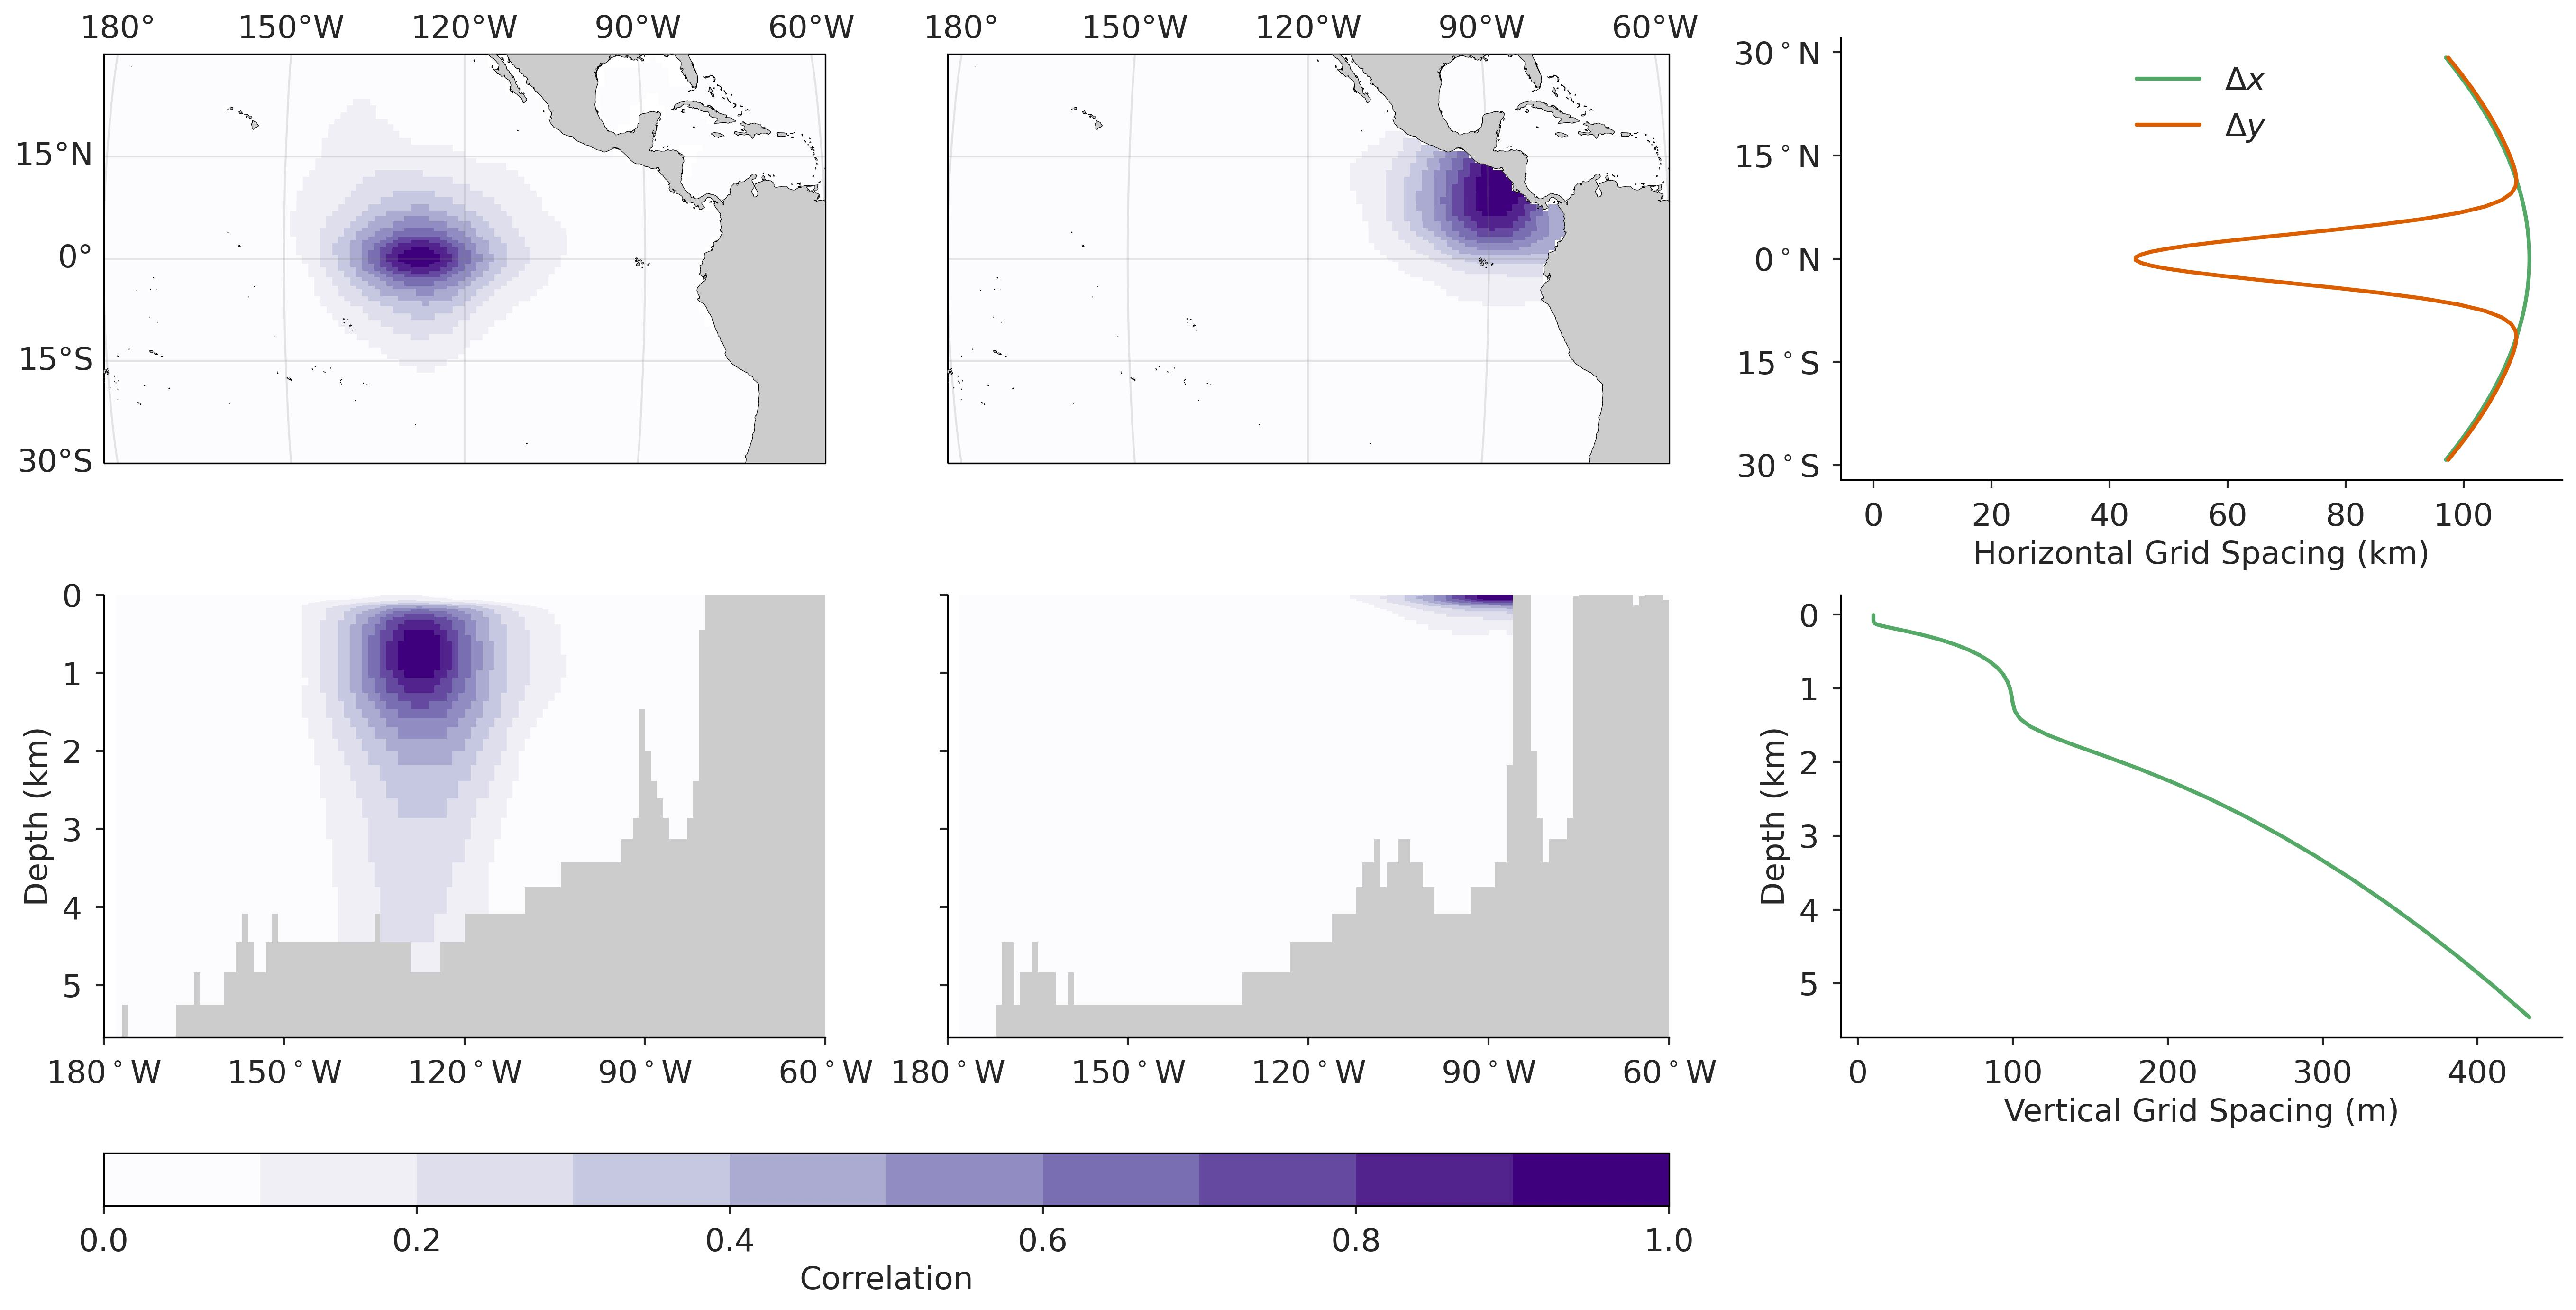
\includegraphics[width=\textwidth]{../figures/huge_correlation_map_02apps.jpg}
    \caption{Two sample correlation fields and a depiction of the computational
        grid.
        (a \& b) Sample correlation field in the latitude-longitude plane at
        (0.2$^\circ$N, 127.5$^\circ$W, 722~m depth) and
        (10.5$^\circ$N, 87.5$^\circ$W, 5~m depth), respectively.
        (c \& d) The same sample correlation fields as above, shown in the
        depth-longitude plane.
        (e \& f) The local horizontal and vertical grid spacing, respectively.
        The sample correlation fields are computed from 1,000 random samples,
        with $\rangeh = 20$ and $M=2$.
    }
    \label{fig:llc90_correlation_maps}
\end{figure}

Panels (d) and (e) of \cref{fig:llc90_correlation_maps} show the extent of the
sample correlation fields from (a) and (b) in depth-longitude space, respectively.
In panel (d) the correlation remains greater than 0.1 until roughly 4-km
depth, whereas the correlation structure in panel (e) is much more confined to
the surface.
Once again, the difference in behavior is due to the fact that the vertical grid
spacing is smaller toward the surface than it is below 1000~m in order to
resolve the ocean mixed layer and surface processes, see
\cref{fig:llc90_correlation_maps}(f).

\subsection{Pointwise sample standard deviation}
\label{ssec:llc90_boundary_effects}


The pointwise, sample standard deviation is shown in \cref{fig:std_ratio}, where
it is represented as a ratio with respect to the ``expected'' value from
\cref{eq:matern_variance} for an isotropic, stationary Mat\'ern field.
Throughout most of the domain, the sample standard deviation is approximately
equal to the theoretical value.
Near continental boundaries the standard deviation is inflated, especially
for large values of $\rangeh$ and in regions of tightly confined topographic
boundaries such as in the Caribbean Sea.
This deviation near the boundaries is expected for correlation models based on
the solution of differential equations
\citep[e.g.][]{weaver_correlation_2001,RSSB:RSSB777}, as a result of the zero
flux, Neumann boundary conditions used to find the solution.
Thus, it is necessary to estimate the sample variance to normalize the
covariance model (i.e.\ formulate the diagonal entries of $\normalizer$,
\cref{eq:matern_operator}), rather than use the theoretical value directly.
Throughout this work, we have used the sample estimates shown in
\cref{fig:std_ratio} to obtain correlation fields.
Given the correspondence to theoretical correlation structure in
\cref{ssec:llc90_correlations}, this appears to be reliable.
Other methods to remove boundary effects, for instance through the
combination of Neumann and Dirichlet boundary conditions as shown for the
implicit diffusion approach in Section 4.2 of
\citet{mirouze_representation_2010}, could be explored in future work.

\begin{figure}
    \centering
    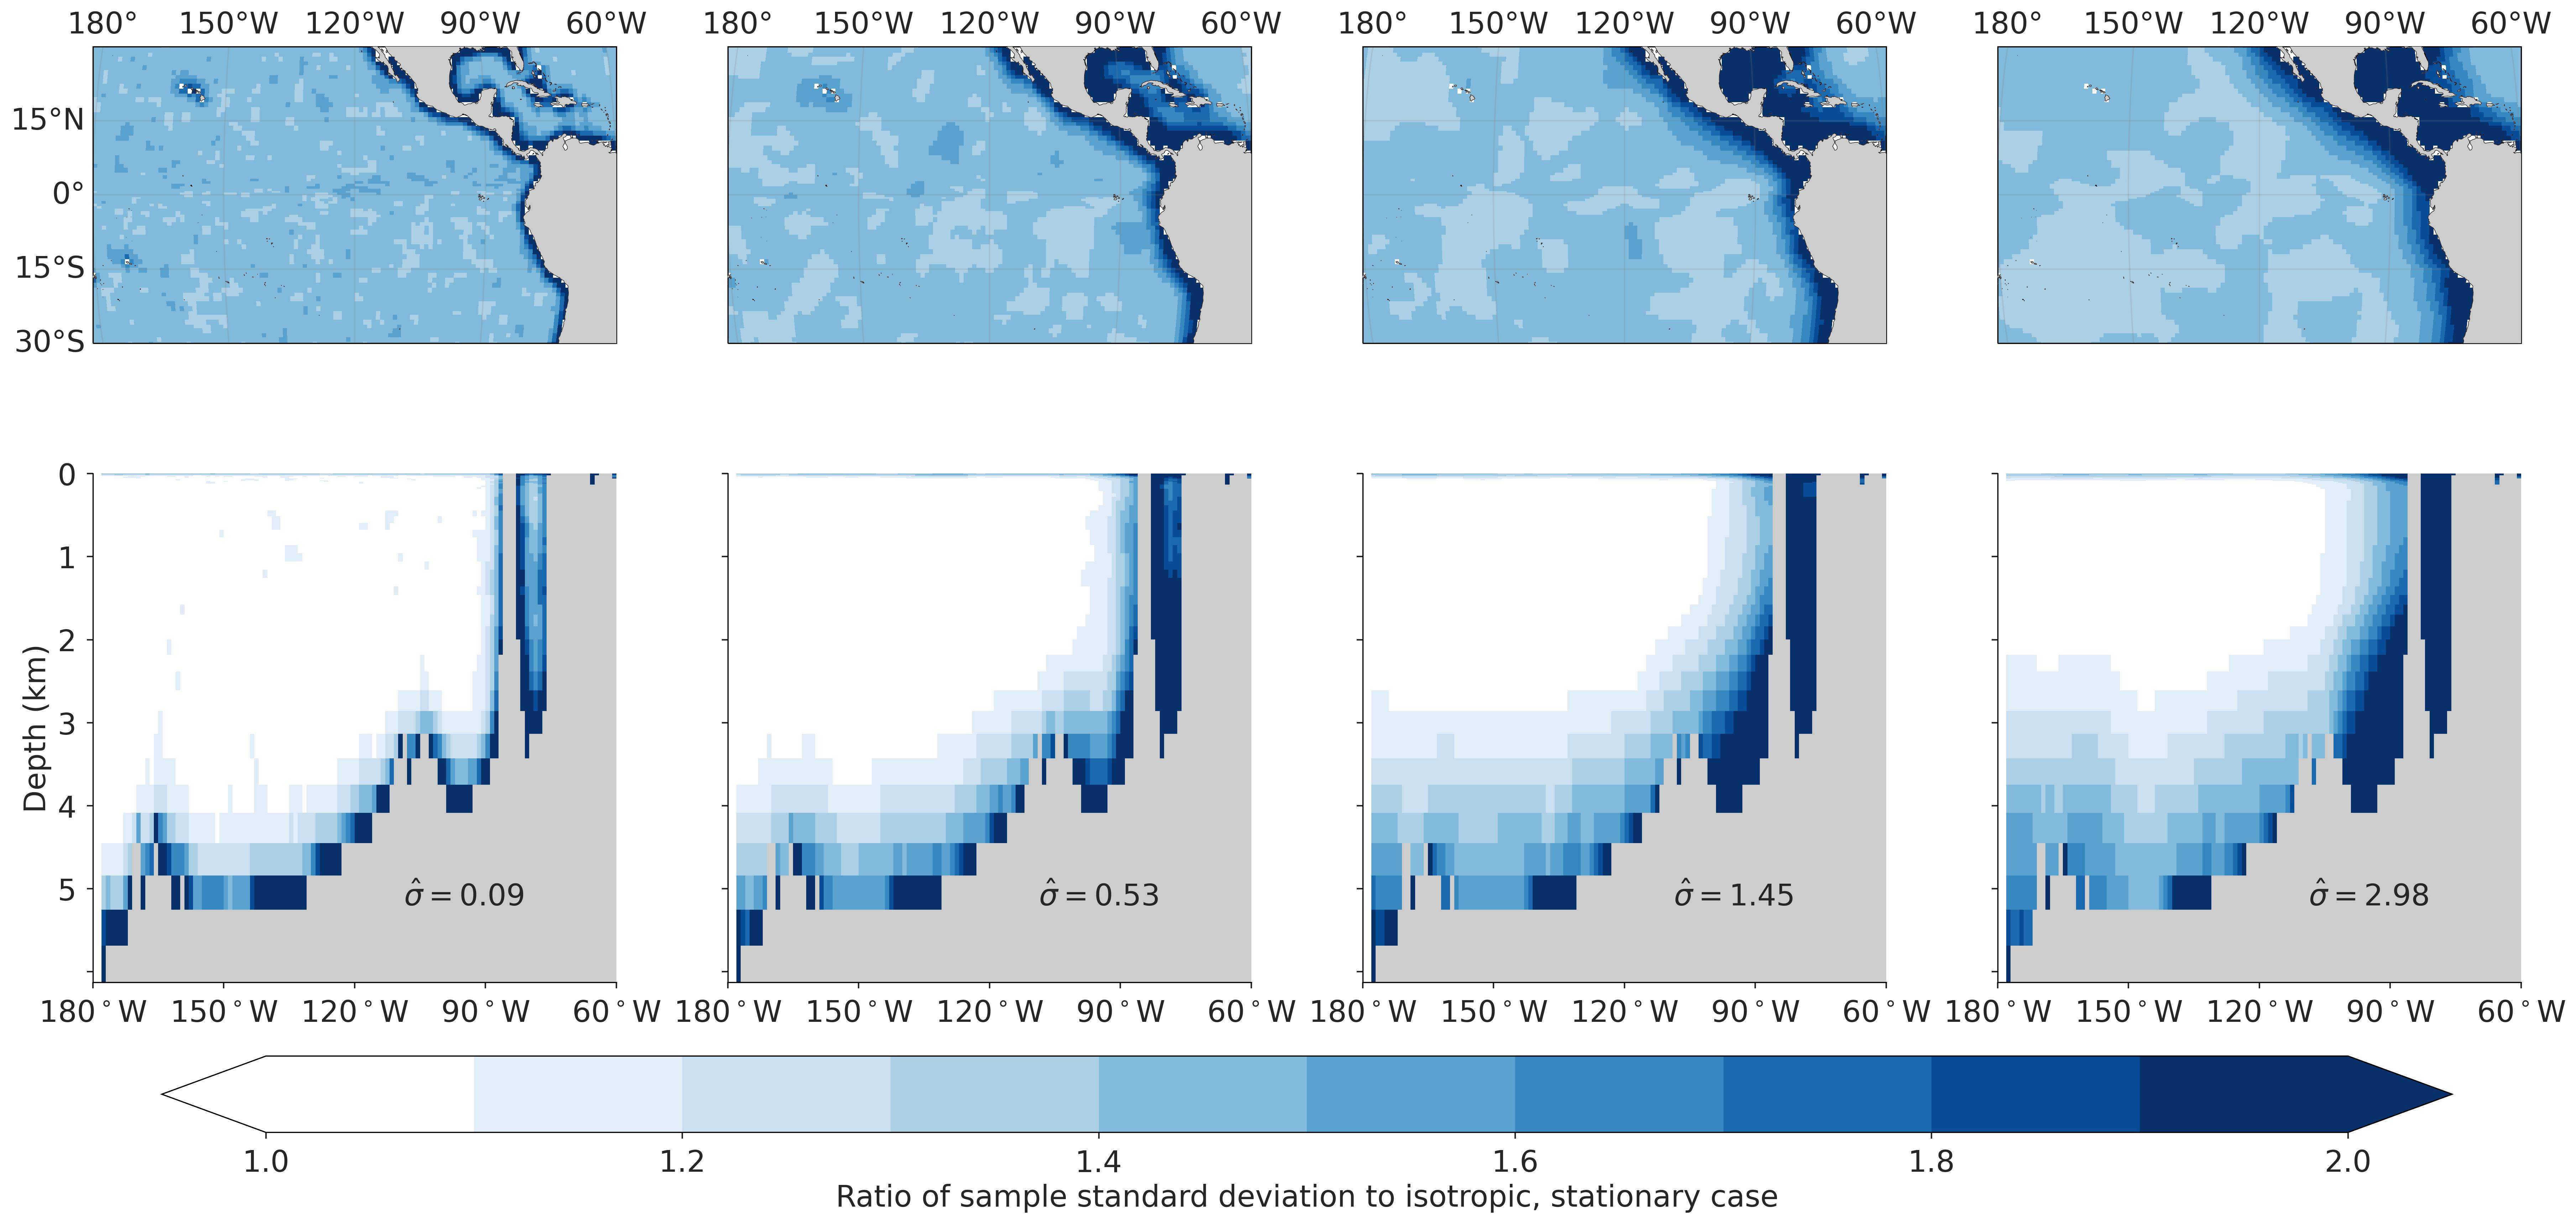
\includegraphics[width=\textwidth]{../figures/std_ratio_02apps.jpg}
    \caption{The ratio of the sample standard deviation to the value computed
        from \cref{eq:matern_variance} for an isotropic, stationary Mat\'ern
        field. Panels (a-d) show the ratio in the latitude-longitude plane at
        the surface for $\rangeh=\{5,10,15,20\}$, respectively. Panels (e-h)
        show the corresponding fields in the depth-longitude plane along 10.5$^\circ$N.
        The largest deviations from the theoretical value are near the boundaries, as
        expected.
        All fields are estimated from 1,000 random samples using $M=2$.
    }
    \label{fig:std_ratio}
\end{figure}

\subsection{High efficiency with low precision}
\label{ssec:tolerance}

The numerical results shown in this section have employed the
iterative algorithm in \cref{sec:block_sor} to obtain approximate correlation
statistics.
As with any iterative algorithm, one must specify a
tolerance that can be used to determine when the algorithm has converged to an
approximate solution.
Within this framework, one can always set a tolerance based on the numerical
precision being used to be confident that the solver has converged.
However, in this section we show that this is likely to be
unnecessarily ambitious.

To be specific, \cref{fig:error_and_iters}(a) shows the relative error in the
approximation that correlation is equal to 0.14 when $\rangeh = \delta i$
for $\rangeh = \{5, 10, 15, 20\}$ (i.e.\ corresponding to the curves in
\cref{fig:llc90_correlations}).
The error in the approximation is shown for a range of solver tolerances,
where $10^{-15}$ is chosen as an approximate lower bound tolerance for double
precision.
For tolerances at $10^{-3}$ and smaller, the error coverges to roughly the same
value, indicating that the desired statistics of the correlation
model are obtained even with a relatively imprecise solve.
We note that \citet{carrier_background-error_2010} describe similar findings
with the implicit diffusion correlation model.

The motivation for using a high tolerance is indicated by
\cref{fig:error_and_iters}(b), which shows how the number of iterations required
to converge increases with the specified tolerance.
Solving to a tolerance of $10^{-15}$ requires a factor of 6-13
more iterations than are required with a tolerance of $10^{-3}$.
Of course, the specific computational savings obtained will depend on the
iterative method that is being used, but we provide this as a concrete example
to highlight that an imprecise solve is both valid and advantageous.

\begin{figure}
    \centering
    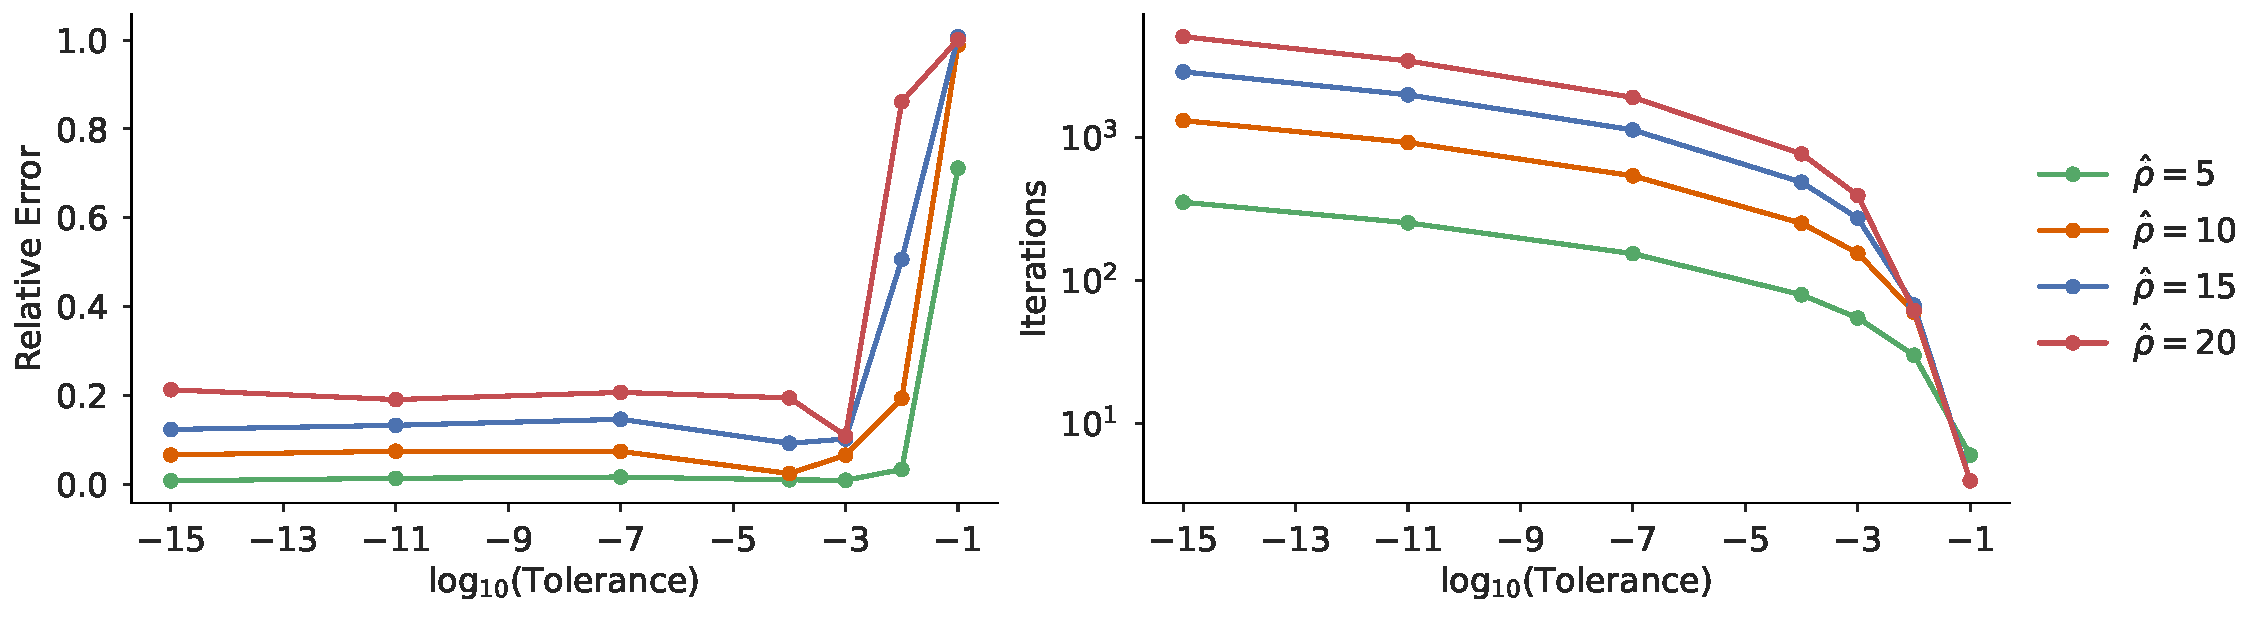
\includegraphics[width=\textwidth]{../figures/matern_llc90_error_and_iters.pdf}
    \caption{(a) The relative error in the approximation that correlation equals
        0.14 when $\rangeh=\delta i$, as a function of the tolerance used
        for the iterative block-SOR method described in \cref{sec:block_sor}.
        Each curve is computed as the error between the theoretical (black)
        curve and the average of each shaded curve shown in \cref{fig:llc90_correlations}.
        (b) The number of iterations required for the block-SOR method to
        converge to the specified tolerance.
        Averages are computed from 1,000 samples using $M=1$.
    }
    \label{fig:error_and_iters}
\end{figure}

\subsection{Rapid convergence for $M>1$}
\label{ssec:iters_and_apps}

For applications where a Gaussian correlation structure is desired, the
correlation model presented here requires $M>1$ to approach the Gaussian
structure (\cref{fig:correlation_comparison}).
Moreover, it could also be desirable to use $\maternop^{-M}$ with $M>1$,
given that $M=1$ produces larger spread in the correlation structure
(\cref{fig:llc90_correlations}(a)), and because the correlation structure drops
off much more rapidly for neighboring points.
For these cases, it may be natural to assume that using this model with $M>1$
would be less efficient than when $M=1$ because it requires multiple
applications of an inverse elliptic operator.
However, here we show that this is evidently not necessarily true and it is
actually often \textit{more} efficient to use $M>1$ than $M=1$.

\cref{fig:iters_and_apps}(a) shows the total number of iterations required to
find a solution to \cref{eq:matern_operator}, for a variety of combinations of
$\rangeh$ and $M$.
Here, ``total iterations'' refers to all block-SOR iterations
required by the algorithm in \cref{sec:block_sor}, summing over all applications
of $\maternop^{-M}$.
Evidently, using $M>1$ actually requires \textit{fewer} total iterations to converge to a
solution than when $M=1$.
The reason for this is as follows.
For any value of $\rangeh$, $\deltah$ increases linearly with $M$, which
increases the amplitude of the diagonal elements of the matrix representation of
$\maternop$.
In each case, the off-diagonal matrix elements, determined by the Laplacian
operator, remain fixed.
Thus, the matrix becomes more diagonally dominant:
the amplitude of the diagonal elements increases relative to the sum total of
off-diagonals.
The degree of diagonal dominance is an important property for
determining the convergence of our SOR-based elliptic solver, where a more
diagonally dominant matrix tends to converge faster \citep{golub_matrix_2013}.
Evidence of this behavior can be seen in \cref{fig:iters_and_apps}(b), which shows the
number of iterations required for each individual application of
$\maternop^{-1}$ to converge.
Here we see that each application gets cheaper as $M$, and therefore $\deltah$,
increases and the improvement per iteration is evidently enough to reduce the total
iterations, shown in panel (a).
The exception to this behavior is when $\rangeh = 5$, where for $M\ge 4$
the total number of iterations overtakes the case of $M=1$ due to the repeated
solves.

\begin{figure}
    \centering
    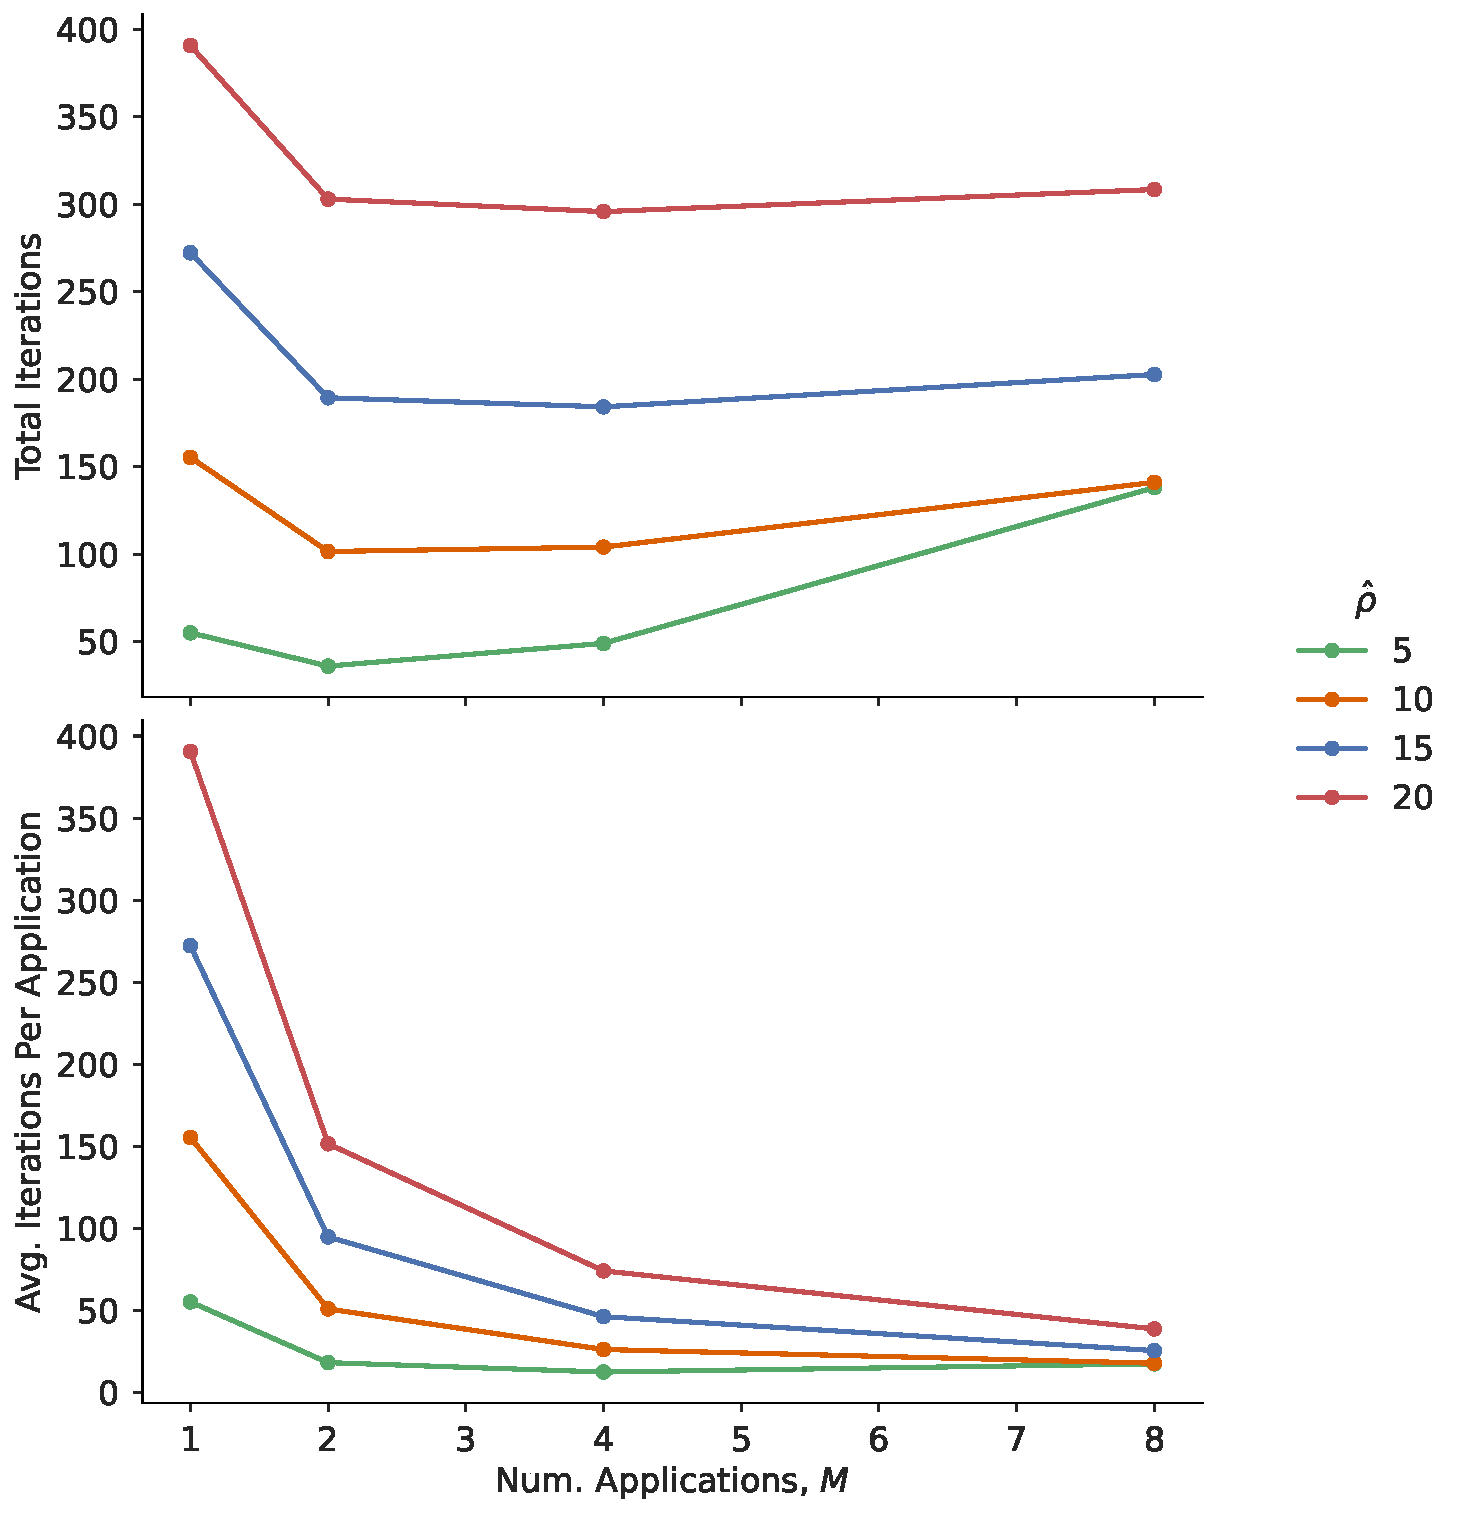
\includegraphics[width=.7\textwidth]{../figures/iterations_vs_applications.pdf}
    \caption{(a) Total number of iterations required to compute
        $\unis = \maternop^{-M}\mathbf{z}$, for a standard normally distributed
        vector $\mathbf{z}\in\ndspace$.
        ``Total iterations'' is represented as the average number of total
        iterations from 1,000 random samples.
        (b) The average number of iterations per application of
        $\maternop^{-M}$, as a function of $M$.
        For all $\rangeh$ and $M$ combinations, each application gets cheaper as
        $M$ increases.
        To compute the ``average iterations per application'', we take the
        average iteration per application of $\maternop^{-M}$, and compute the sample
        average of this quantity from 1,000 random samples.
        Solver tolerance is set to $10^{-3}$.
    }
    \label{fig:iters_and_apps}
\end{figure}
